%============================================================
% MTH 112 Project - Angles
% Updated 202504
%============================================================

\section{The Unit Circle Supplemental Questions} \label{supplement-unit-circle}
In this section, you can practice answering some extra questions about the topics in this chapter.

\subsection*{Practice Exercises} \label{practice-exercises-supplement}

\begin{myPractice}
	Explain why exactly $2\pi$ radians measure the full angle inside a circle.
	\vfill
\end{myPractice}

\begin{myPractice}
	\begin{multicols}{2}
		Use \say{SOHCAHTOA} and \say {CHOSHACAO} to find the following values for the triangle in Figure \ref{supplement-section-right-triangle-trig-example-triangle}.
		\columnbreak
		\begin{center}\captionsetup{type=figure} \captionof{figure}{A right triangle}
			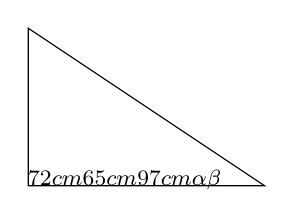
\begin{tikzpicture}[thin] \label{supplement-section-right-triangle-trig-example-triangle}
				\coordinate (O) at (0,0);
				\coordinate (A) at (3,0);
				\coordinate (B) at (0,2);
				\draw (O)--(A)--(B)--cycle;
				\footnotesize
				\tkzLabelSegment[below=2pt](O,A){$72\text{cm}$}
				\tkzLabelSegment[above=2pt,rotate=90](O,B){$65\text{cm}$}
				\tkzLabelSegment[above=2pt, rotate=-atan(2/3)](A,B){$97\text{cm}$}
				\tkzMarkRightAngle[size=0.5](A,O,B)
				\tkzMarkAngle[size=0.8cm](B,A,O)
				\tkzLabelAngle[pos = 0.6](B,A,O){$\alpha$}
				\tkzMarkAngle[size=0.7cm](O,B,A)
				\tkzLabelAngle[pos = 0.5](O,B,A){$\beta$}
			\end{tikzpicture}
		\end{center}
	\end{multicols}
	\begin{multicols}{4}
		\begin{enumerate}
			\item $\sin(\alpha)$
			\vspace{2cm}
			\item $\cos(\alpha)$
			\vspace{2cm}
			\item $\tan(\alpha)$
			\vspace{2cm}
			\item $\sin(\beta)$
			\vspace{2cm}
			\item $\cos(\beta)$
			\vspace{2cm}
			\item $\tan(\beta)$
			\vspace{2cm}
			\item $\csc(\alpha)$
			\vspace{2cm}
			\item $\sec(\alpha)$
			\vspace{2cm}
			\item $\cot(\alpha)$
			\vspace{2cm}
			\item $\csc(\beta)$
			\vspace{2cm}
			\item $\sec(\beta)$
			\vspace{2cm}
			\item $\cot(\beta)$
			\vspace{2cm}
		\end{enumerate}
	\end{multicols}
\end{myPractice}